\upaper{79}{Andite Expansion in the Orient}
\author{Archangel}
\vs p079 0:1 Asia is the homeland of the human race. It was on a southern peninsula of this continent that Andon and Fonta were born; in the highlands of what is now Afghanistan, their descendant Badonan founded a primitive centre of culture that persisted for over 500,000 years. Here at this eastern focus of the human race the Sangik peoples differentiated from the Andonic stock, and Asia was their first home, their first hunting ground, their first battlefield. South\hyp{}western Asia witnessed the successive civilizations of Dalamatians, Nodites, Adamites, and Andites, and from these regions the potentials of modern civilization spread to the world.
\usection{1.\bibnobreakspace The Andites of Turkestan}
\vs p079 1:1 For over 25,000 years, on down to nearly 2000\,B.C., the heart of Eurasia was predominantly, though diminishingly, Andite. In the lowlands of Turkestan the Andites made the westward turning around the inland lakes into Europe, while from the highlands of this region they infiltrated eastward. Eastern Turkestan (Sinkiang) and, to a lesser extent, Tibet were the ancient gateways through which these peoples of Mesopotamia penetrated the mountains to the northern lands of the yellow men. The Andite infiltration of India proceeded from the Turkestan highlands into the Punjab and from the Iranian grazing lands through Baluchistan. These earlier migrations were in no sense conquests; they were, rather, the continual drifting of the Andite tribes into western India and China.
\vs p079 1:2 \pc For almost 15,000 years centres of mixed Andite culture persisted in the basin of the Tarim River in Sinkiang and to the south in the highland regions of Tibet, where the Andites and Andonites had extensively mingled. The Tarim valley was the easternmost outpost of the true Andite culture. Here they built their settlements and entered into trade relations with the progressive Chinese to the east and with the Andonites to the north. In those days the Tarim region was a fertile land; the rainfall was plentiful. To the east the Gobi was an open grassland where the herders were gradually turning to agriculture. This civilization perished when the rain winds shifted to the south\hyp{}east, but in its day it rivalled Mesopotamia itself.
\vs p079 1:3 \pc By 8000\,B.C. the slowly increasing aridity of the highland regions of central Asia began to drive the Andites to the river bottoms and the seashores. This increasing drought not only drove them to the valleys of the Nile, Euphrates, Indus, and Yellow rivers, but it produced a new development in Andite civilization. A new class of men, the traders, began to appear in large numbers.
\vs p079 1:4 When climatic conditions made hunting unprofitable for the migrating Andites, they did not follow the evolutionary course of the older races by becoming herders. Commerce and urban life made their appearance. From Egypt through Mesopotamia and Turkestan to the rivers of China and India, the more highly civilized tribes began to assemble in cities devoted to manufacture and trade. Adonia became the central Asian commercial metropolis, being located near the present city of Ashkhabad. Commerce in stone, metal, wood, and pottery was accelerated on both land and water.
\vs p079 1:5 But ever\hyp{}increasing drought gradually brought about the great Andite exodus from the lands south and east of the Caspian Sea. The tide of migration began to veer from northward to southward, and the Babylonian cavalrymen began to push into Mesopotamia.
\vs p079 1:6 Increasing aridity in central Asia further operated to reduce population and to render these people less warlike; and when the diminishing rainfall to the north forced the nomadic Andonites southward, there was a tremendous exodus of Andites from Turkestan. This is the terminal movement of the so\hyp{}called Aryans into the Levant and India. It culminated that long dispersal of the mixed descendants of Adam during which every Asiatic and most of the island peoples of the Pacific were to some extent improved by these superior races.
\vs p079 1:7 Thus, while they dispersed over the Eastern Hemisphere, the Andites were dispossessed of their homelands in Mesopotamia and Turkestan, for it was this extensive southward movement of Andonites that diluted the Andites in central Asia nearly to the vanishing point.
\vs p079 1:8 But even in the XX century after Christ there are traces of Andite blood among the Turanian and Tibetan peoples, as is witnessed by the blond types occasionally found in these regions. The early Chinese annals record the presence of the red\hyp{}haired nomads to the north of the peaceful settlements of the Yellow River, and there still remain paintings which faithfully record the presence of both the blond\hyp{}Andite and the brunet\hyp{}Mongolian types in the Tarim basin of long ago.
\vs p079 1:9 The last great manifestation of the submerged military genius of the central Asiatic Andites was in A.D.\,1200, when the Mongols under Genghis Khan began the conquest of the greater portion of the Asiatic continent. And like the Andites of old, these warriors proclaimed the existence of “one God in heaven.” The early breakup of their empire long delayed cultural intercourse between Occident and Orient and greatly handicapped the growth of the monotheistic concept in Asia.
\usection{2.\bibnobreakspace The Andite Conquest of India}
\vs p079 2:1 India is the only locality where all the Urantia races were blended, the Andite invasion adding the last stock. In the highlands north\hyp{}west of India the Sangik races came into existence, and without exception members of each penetrated the subcontinent of India in their early days, leaving behind them the most heterogeneous race mixture ever to exist on Urantia. Ancient India acted as a catch basin for the migrating races. The base of the peninsula was formerly somewhat narrower than now, much of the deltas of the Ganges and Indus being the work of the last 50,000 years.
\vs p079 2:2 The earliest race mixtures in India were a blending of the migrating red and yellow races with the aboriginal Andonites. This group was later weakened by absorbing the greater portion of the extinct eastern green peoples as well as large numbers of the orange race, was slightly improved through limited admixture with the blue man, but suffered exceedingly through assimilation of large numbers of the indigo race. But the so\hyp{}called aborigines of India are hardly representative of these early people; they are rather the most inferior southern and eastern fringe, which was never fully absorbed by either the early Andites or their later appearing Aryan cousins.
\vs p079 2:3 \pc By 20,000\,B.C. the population of western India had already become tinged with the Adamic blood, and never in the history of Urantia did any one people combine so many different races. But it was unfortunate that the secondary Sangik strains predominated, and it was a real calamity that both the blue and the red man were so largely missing from this racial melting pot of long ago; more of the primary Sangik strains would have contributed very much toward the enhancement of what might have been an even greater civilization. As it developed, the red man was destroying himself in the Americas, the blue man was disporting himself in Europe, and the early descendants of Adam (and most of the later ones) exhibited little desire to admix with the darker coloured peoples, whether in India, Africa, or elsewhere.
\vs p079 2:4 \pc About 15,000\,B.C. increasing population pressure throughout Turkestan and Iran occasioned the first really extensive Andite movement toward India. For over 15 centuries these superior peoples poured in through the highlands of Baluchistan, spreading out over the valleys of the Indus and Ganges and slowly moving southward into the Deccan. This Andite pressure from the north\hyp{}west drove many of the southern and eastern inferiors into Burma and southern China but not sufficiently to save the invaders from racial obliteration.
\vs p079 2:5 The failure of India to achieve the hegemony of Eurasia was largely a matter of topography; population pressure from the north only crowded the majority of the people southward into the decreasing territory of the Deccan, surrounded on all sides by the sea. Had there been adjacent lands for emigration, then would the inferiors have been crowded out in all directions, and the superior stocks would have achieved a higher civilization.
\vs p079 2:6 As it was, these earlier Andite conquerors made a desperate attempt to preserve their identity and stem the tide of racial engulfment by the establishment of rigid restrictions regarding intermarriage. Nonetheless, the Andites had become submerged by 10,000\,B.C., but the whole mass of the people had been markedly improved by this absorption.
\vs p079 2:7 \pc Race mixture is always advantageous in that it favours versatility of culture and makes for a progressive civilization, but if the inferior elements of racial stocks predominate, such achievements will be short\hyp{}lived. A polyglot culture can be preserved only if the superior stocks reproduce themselves in a safe margin over the inferior. Unrestrained multiplication of inferiors, with decreasing reproduction of superiors, is unfailingly suicidal of cultural civilization.
\vs p079 2:8 Had the Andite conquerors been in numbers three times what they were, or had they driven out or destroyed the least desirable third of the mixed orange\hyp{}green\hyp{}indigo inhabitants, then would India have become one of the world’s leading centres of cultural civilization and undoubtedly would have attracted more of the later waves of Mesopotamians that flowed into Turkestan and thence northward to Europe.
\usection{3.\bibnobreakspace Dravidian India}
\vs p079 3:1 The blending of the Andite conquerors of India with the native stock eventually resulted in that mixed people which has been called Dravidian. The earlier and purer Dravidians possessed a great capacity for cultural achievement, which was continuously weakened as their Andite inheritance became progressively attenuated. And this is what doomed the budding civilization of India almost 12,000 years ago. But the infusion of even this small amount of the blood of Adam produced a marked acceleration in social development. This composite stock immediately produced the most versatile civilization then on earth.
\vs p079 3:2 Not long after conquering India, the Dravidian Andites lost their racial and cultural contact with Mesopotamia, but the later opening up of the sea lanes and the caravan routes re\hyp{}established these connections; and at no time within the last 10,000 years has India ever been entirely out of touch with Mesopotamia on the west and China to the east, although the mountain barriers greatly favoured western intercourse.
\vs p079 3:3 \pc The superior culture and religious leanings of the peoples of India date from the early times of Dravidian domination and are due, in part, to the fact that so many of the Sethite priesthood entered India, both in the earlier Andite and in the later Aryan invasions. The thread of monotheism running through the religious history of India thus stems from the teachings of the Adamites in the second garden.
\vs p079 3:4 As early as 16,000\,B.C. a company of 100 Sethite priests entered India and very nearly achieved the religious conquest of the western half of that polyglot people. But their religion did not persist. Within 5,000 years their doctrines of the Paradise Trinity had degenerated into the triune symbol of the fire god.
\vs p079 3:5 But for more than 7,000 years, down to the end of the Andite migrations, the religious status of the inhabitants of India was far above that of the world at large. During these times India bid fair to produce the leading cultural, religious, philosophic, and commercial civilization of the world. And but for the complete submergence of the Andites by the peoples of the south, this destiny would probably have been realized.
\vs p079 3:6 \pc The Dravidian centres of culture were located in the river valleys, principally of the Indus and Ganges, and in the Deccan along the three great rivers flowing through the Eastern Ghats to the sea. The settlements along the seacoast of the Western Ghats owed their prominence to maritime relationships with Sumeria.
\vs p079 3:7 The Dravidians were among the earliest peoples to build cities and to engage in an extensive export and import business, both by land and sea. By 7000\,B.C. camel trains were making regular trips to distant Mesopotamia; Dravidian shipping was pushing coastwise across the Arabian Sea to the Sumerian cities of the Persian Gulf and was venturing on the waters of the Bay of Bengal as far as the East Indies. An alphabet, together with the art of writing, was imported from Sumeria by these seafarers and merchants.
\vs p079 3:8 These commercial relationships greatly contributed to the further diversification of a cosmopolitan culture, resulting in the early appearance of many of the refinements and even luxuries of urban life. When the later appearing Aryans entered India, they did not recognize in the Dravidians their Andite cousins submerged in the Sangik races, but they did find a well\hyp{}advanced civilization. Despite biologic limitations, the Dravidians founded a superior civilization. It was well diffused throughout all India and has survived on down to modern times in the Deccan.
\usection{4.\bibnobreakspace The Aryan Invasion of India}
\vs p079 4:1 The second Andite penetration of India was the Aryan invasion during a period of almost 500 years in the middle of the third millennium before Christ. This migration marked the terminal exodus of the Andites from their homelands in Turkestan.
\vs p079 4:2 The early Aryan centres were scattered over the northern half of India, notably in the north\hyp{}west. These invaders never completed the conquest of the country and subsequently met their undoing in this neglect since their lesser numbers made them vulnerable to absorption by the Dravidians of the south, who subsequently overran the entire peninsula except the Himalayan provinces.
\vs p079 4:3 The Aryans made very little racial impression on India except in the northern provinces. In the Deccan their influence was cultural and religious more than racial. The greater persistence of the so\hyp{}called Aryan blood in northern India is not only due to their presence in these regions in greater numbers but also because they were reinforced by later conquerors, traders, and missionaries. Right on down to the first century before Christ there was a continuous infiltration of Aryan blood into the Punjab, the last influx being attendant upon the campaigns of the Hellenistic peoples.\tunemarkup{pictures}{\begin{figure}[H]\centering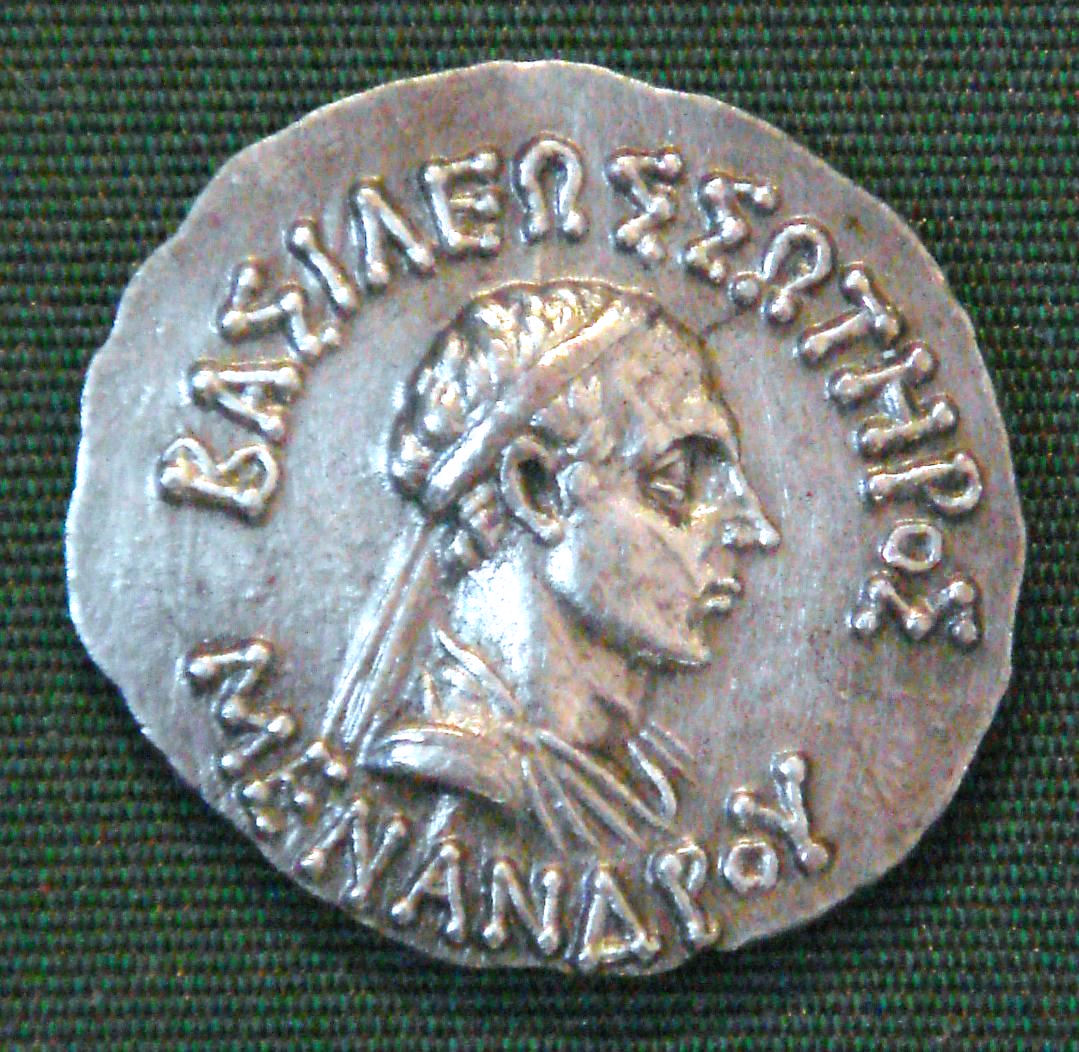
\includegraphics[width=0.6\columnwidth]{images/MenandrosCoin.jpg}\caption{Menander I Soter (165/155--130 BCE), conqueror of the Punjab, carved out a Greek kingdom in the Punjab and ruled the Punjab until his death in 130 BC.}\end{figure}}
\vs p079 4:4 On the Gangetic plain Aryan and Dravidian eventually mingled to produce a high culture, and this centre was later reinforced by contributions from the north\hyp{}east, coming from China.
\vs p079 4:5 In India many types of social organizations flourished from time to time, from the semidemocratic systems of the Aryans to despotic and monarchial forms of government. But the most characteristic feature of society was the persistence of the great social castes that were instituted by the Aryans in an effort to perpetuate racial identity. This elaborate caste system has been preserved on down to the present time.
\vs p079 4:6 Of the four great castes, all but the first were established in the futile effort to prevent racial amalgamation of the Aryan conquerors with their inferior subjects. But the premier caste, the teacher\hyp{}priests, stems from the Sethites; the Brahmans of the XX century after Christ are the lineal cultural descendants of the priests of the second garden, albeit their teachings differ greatly from those of their illustrious predecessors.
\vs p079 4:7 When the Aryans entered India, they brought with them their concepts of Deity as they had been preserved in the lingering traditions of the religion of the second garden. But the Brahman priests were never able to withstand the pagan momentum built up by the sudden contact with the inferior religions of the Deccan after the racial obliteration of the Aryans. Thus the vast majority of the population fell into the bondage of the enslaving superstitions of inferior religions; and so it was that India failed to produce the high civilization which had been foreshadowed in earlier times.
\vs p079 4:8 The spiritual awakening of the VI century before Christ did not persist in India, having died out even before the Mohammedan invasion. But someday a greater Gautama may arise to lead all India in the search for the living God, and then the world will observe the fruition of the cultural potentialities of a versatile people so long comatose under the benumbing influence of an unprogressing spiritual vision.
\vs p079 4:9 Culture does rest on a biologic foundation, but caste alone could not perpetuate the Aryan culture, for religion, true religion, is the indispensable source of that higher energy which drives men to establish a superior civilization based on human brotherhood.
\usection{5.\bibnobreakspace Red Man and Yellow Man}
\vs p079 5:1 While the story of India is that of Andite conquest and eventual submergence in the older evolutionary peoples, the narrative of eastern Asia is more properly that of the primary Sangiks, particularly the red man and the yellow man. These two races largely escaped that admixture with the debased Neanderthal strain which so greatly retarded the blue man in Europe, thus preserving the superior potential of the primary Sangik type.
\vs p079 5:2 While the early Neanderthalers were spread out over the entire breadth of Eurasia, the eastern wing was the more contaminated with debased animal strains. These subhuman types were pushed south by the fifth glacier, the same ice sheet which so long blocked Sangik migration into eastern Asia. And when the red man moved north\hyp{}east around the highlands of India, he found north\hyp{}eastern Asia free from these subhuman types. The tribal organization of the red races was formed earlier than that of any other peoples, and they were the first to migrate from the central Asian focus of the Sangiks. The inferior Neanderthal strains were destroyed or driven off the mainland by the later migrating yellow tribes. But the red man had reigned supreme in eastern Asia for almost 100,000 years before the yellow tribes arrived.
\vs p079 5:3 \pc More than 300,000 years ago the main body of the yellow race entered China from the south as coastwise migrants. Each millennium they penetrated farther and farther inland, but they did not make contact with their migrating Tibetan brethren until comparatively recent times.
\vs p079 5:4 Growing population pressure caused the northward\hyp{}moving yellow race to begin to push into the hunting grounds of the red man. This encroachment, coupled with natural racial antagonism, culminated in increasing hostilities, and thus began the crucial struggle for the fertile lands of farther Asia.
\vs p079 5:5 The story of this agelong contest between the red and yellow races is an epic of Urantia history. For over 200,000 years these two superior races waged bitter and unremitting warfare. In the earlier struggles the red men were generally successful, their raiding parties spreading havoc among the yellow settlements. But the yellow man was an apt pupil in the art of warfare, and he early manifested a marked ability to live peaceably with his compatriots; the Chinese were the first to learn that in union there is strength. The red tribes continued their internecine conflicts, and presently they began to suffer repeated defeats at the aggressive hands of the relentless Chinese, who continued their inexorable march northward.
\vs p079 5:6 \pc 100,000 years ago the decimated tribes of the red race were fighting with their backs to the retreating ice of the last glacier, and when the land passage to the West\fnc{the land passage to the \bibtextul{west,} over the Bering isthmus\ldots{} \bibexpl{The change from “west” to “east,” as found in many printings, is geographically correct but typographically impossible; the committee adopted the alternate “West” referring to the Western Hemisphere --- the word thus indicating a place rather than a direction of travel.}}, over the Bering isthmus, became passable, these tribes were not slow in forsaking the inhospitable shores of the Asiatic continent. It is 85,000 years since the last of the pure red men departed from Asia, but the long struggle left its genetic imprint upon the victorious yellow race. The northern Chinese peoples, together with the Andonite Siberians, assimilated much of the red stock and were in considerable measure benefited thereby.
\vs p079 5:7 The North American Indians never came in contact with even the Andite offspring of Adam and Eve, having been dispossessed of their Asiatic homelands some 50,000 years before the coming of Adam. During the age of Andite migrations the pure red strains were spreading out over North America as nomadic tribes, hunters who practised agriculture to a small extent. These races and cultural groups remained almost completely isolated from the remainder of the world from their arrival in the Americas down to the end of the first millennium of the Christian era, when they were discovered by the white races of Europe. Up to that time the Eskimos were the nearest to white men the northern tribes of red men had ever seen.
\vs p079 5:8 The red and the yellow races are the only human stocks that ever achieved a high degree of civilization apart from the influences of the Andites. The oldest Amerindian culture was the Onamonalonton centre in California, but this had long since vanished by 35,000\,B.C. In Mexico, Central America, and in the mountains of South America the later and more enduring civilizations were founded by a race predominantly red but containing a considerable admixture of the yellow, orange, and blue.
\vs p079 5:9 These civilizations were evolutionary products of the Sangiks, notwithstanding that traces of Andite blood reached Peru. Excepting the Eskimos in North America and a few Polynesian Andites in South America, the peoples of the Western Hemisphere had no contact with the rest of the world until the end of the first millennium after Christ. In the original Melchizedek plan for the improvement of the Urantia races it had been stipulated that 1,000,000 of the pure\hyp{}line descendants of Adam should go to upstep the red men of the Americas.
\usection{6.\bibnobreakspace Dawn of Chinese Civilization}
\vs p079 6:1 Sometime after driving the red man across to North America, the expanding Chinese cleared the Andonites from the river valleys of eastern Asia, pushing them north into Siberia and west into Turkestan, where they were soon to come in contact with the superior culture of the Andites.
\vs p079 6:2 In Burma and the peninsula of Indo\hyp{}China the cultures of India and China mixed and blended to produce the successive civilizations of those regions. Here the vanished green race has persisted in larger proportion than anywhere else in the world.
\vs p079 6:3 Many different races occupied the islands of the Pacific. In general, the southern and then more extensive islands were occupied by peoples carrying a heavy percentage of green and indigo blood. The northern islands were held by Andonites and, later on, by races embracing large proportions of the yellow and red stocks. The ancestors of the Japanese people were not driven off the mainland until 12,000\,B.C., when they were dislodged by a powerful southern\hyp{}coastwise thrust of the northern Chinese tribes. Their final exodus was not so much due to population pressure as to the initiative of a chieftain whom they came to regard as a divine personage.
\vs p079 6:4 Like the peoples of India and the Levant, victorious tribes of the yellow man established their earliest centres along the coast and up the rivers. The coastal settlements fared poorly in later years as the increasing floods and the shifting courses of the rivers made the lowland cities untenable.
\vs p079 6:5 20,000 years ago the ancestors of the Chinese had built up a dozen strong centres of primitive culture and learning, especially along the Yellow River and the Yangtze. And now these centres began to be reinforced by the arrival of a steady stream of superior blended peoples from Sinkiang and Tibet. The migration from Tibet to the Yangtze valley was not so extensive as in the north, neither were the Tibetan centres so advanced as those of the Tarim basin. But both movements carried a certain amount of Andite blood eastward to the river settlements.
\vs p079 6:6 The superiority of the ancient yellow race was due to four great factors:
\vs p079 6:7 \ublistelem{1.}\bibnobreakspace \bibemph{Genetic.} Unlike their blue cousins in Europe, both the red and yellow races had largely escaped mixture with debased human stocks. The northern Chinese, already strengthened by small amounts of the superior red and Andonic strains, were soon to benefit by a considerable influx of Andite blood. The southern Chinese did not fare so well in this regard, and they had long suffered from absorption of the green race, while later on they were to be further weakened by the infiltration of the swarms of inferior peoples crowded out of India by the Dravidian\hyp{}Andite invasion. And today in China there is a definite difference between the northern and southern races.
\vs p079 6:8 \ublistelem{2.}\bibnobreakspace \bibemph{Social.} The yellow race early learned the value of peace among themselves. Their internal peaceableness so contributed to population increase as to ensure the spread of their civilization among many millions. From 25,000 to 5000\,B.C. the highest mass civilization on Urantia was in central and northern China. The yellow man was first to achieve a racial solidarity --- the first to attain a large\hyp{}scale cultural, social, and political civilization.
\vs p079 6:9 The Chinese of 15,000\,B.C. were aggressive militarists; they had not been weakened by an overreverence for the past, and numbering less than 12,000,000, they formed a compact body speaking a common language. During this age they built up a real nation, much more united and homogeneous than their political unions of historic times.
\vs p079 6:10 \ublistelem{3.}\bibnobreakspace \bibemph{Spiritual.} During the age of Andite migrations the Chinese were among the more spiritual peoples of earth. Long adherence to the worship of the One Truth proclaimed by Singlangton kept them ahead of most of the other races. The stimulus of a progressive and advanced religion is often a decisive factor in cultural development; as India languished, so China forged ahead under the invigorating stimulus of a religion in which truth was enshrined as the supreme Deity.
\vs p079 6:11 This worship of truth was provocative of research and fearless exploration of the laws of nature and the potentials of mankind. The Chinese of even 6,000 years ago were still keen students and aggressive in their pursuit of truth.
\vs p079 6:12 \ublistelem{4.}\bibnobreakspace \bibemph{Geographic.} China is protected by the mountains to the west and the Pacific to the east. Only in the north is the way open to attack, and from the days of the red man to the coming of the later descendants of the Andites, the north was not occupied by any aggressive race.
\vs p079 6:13 And but for the mountain barriers and the later decline in spiritual culture, the yellow race undoubtedly would have attracted to itself the larger part of the Andite migrations from Turkestan and unquestionably would have quickly dominated world civilization.
\usection{7.\bibnobreakspace The Andites Enter China}
\vs p079 7:1 About 15,000 years ago the Andites, in considerable numbers, were traversing the pass of Ti Tao and spreading out over the upper valley of the Yellow River among the Chinese settlements of Kansu. Presently they penetrated eastward to Honan, where the most progressive settlements were situated. This infiltration from the west was about half Andonite and half Andite.
\vs p079 7:2 The northern centres of culture along the Yellow River had always been more progressive than the southern settlements on the Yangtze. Within a few thousand years after the arrival of even the small numbers of these superior mortals, the settlements along the Yellow River had forged ahead of the Yangtze villages and had achieved an advanced position over their brethren in the south which has ever since been maintained.
\vs p079 7:3 \pc It was not that there were so many of the Andites, nor that their culture was so superior, but amalgamation with them produced a more versatile stock. The northern Chinese received just enough of the Andite strain to mildly stimulate their innately able minds but not enough to fire them with the restless, exploratory curiosity so characteristic of the northern white races. This more limited infusion of Andite inheritance was less disturbing to the innate stability of the Sangik type.
\vs p079 7:4 \pc The later waves of Andites brought with them certain of the cultural advances of Mesopotamia; this is especially true of the last waves of migration from the west. They greatly improved the economic and educational practices of the northern Chinese; and while their influence upon the religious culture of the yellow race was short\hyp{}lived, their later descendants contributed much to a subsequent spiritual awakening. But the Andite traditions of the beauty of Eden and Dalamatia did influence Chinese traditions; early Chinese legends place “the land of the gods” in the west.
\vs p079 7:5 The Chinese people did not begin to build cities and engage in manufacture until after 10,000\,B.C., subsequent to the climatic changes in Turkestan and the arrival of the later Andite immigrants. The infusion of this new blood did not add so much to the civilization of the yellow man as it stimulated the further and rapid development of the latent tendencies of the superior Chinese stocks. From Honan to Shensi the potentials of an advanced civilization were coming to fruit. Metalworking and all the arts of manufacture date from these days.
\vs p079 7:6 The similarities between certain of the early Chinese and Mesopotamian methods of time reckoning, astronomy, and governmental administration were due to the commercial relationships between these two remotely situated centres. Chinese merchants travelled the overland routes through Turkestan to Mesopotamia even in the days of the Sumerians. Nor was this exchange one\hyp{}sided --- the valley of the Euphrates benefited considerably thereby, as did the peoples of the Gangetic plain. But the climatic changes and the nomadic invasions of the third millennium before Christ greatly reduced the volume of trade passing over the caravan trails of central Asia.
\usection{8.\bibnobreakspace Later Chinese Civilization}
\vs p079 8:1 While the red man suffered from too much warfare, it is not altogether amiss to say that the development of statehood among the Chinese was delayed by the thoroughness of their conquest of Asia. They had a great potential of racial solidarity, but it failed properly to develop because the continuous driving stimulus of the ever\hyp{}present danger of external aggression was lacking.
\vs p079 8:2 With the completion of the conquest of eastern Asia the ancient military state gradually disintegrated --- past wars were forgotten. Of the epic struggle with the red race there persisted only the hazy tradition of an ancient contest with the archer peoples. The Chinese early turned to agricultural pursuits, which contributed further to their pacific tendencies, while a population well below the land\hyp{}man ratio for agriculture still further contributed to the growing peacefulness of the country.
\vs p079 8:3 Consciousness of past achievements (somewhat diminished in the present), the conservatism of an overwhelmingly agricultural people, and a well\hyp{}developed family life equalled the birth of ancestor veneration, culminating in the custom of so honouring the men of the past as to border on worship. A very similar attitude prevailed among the white races in Europe for some 500 years following the disruption of Gr\ae co\hyp{}Roman civilization.
\vs p079 8:4 The belief in, and worship of, the “One Truth” as taught by Singlangton never entirely died out; but as time passed, the search for new and higher truth became overshadowed by a growing tendency to venerate that which was already established. Slowly the genius of the yellow race became diverted from the pursuit of the unknown to the preservation of the known. And this is the reason for the stagnation of what had been the world’s most rapidly progressing civilization.
\vs p079 8:5 \pc Between 4000 and 500\,B.C. the political reunification of the yellow race was consummated, but the cultural union of the Yangtze and Yellow river centres had already been effected. This political reunification of the later tribal groups was not without conflict, but the societal opinion of war remained low; ancestor worship, increasing dialects, and no call for military action for thousands upon thousands of years had rendered this people ultrapeaceful.
\vs p079 8:6 Despite failure to fulfil the promise of an early development of advanced statehood, the yellow race did progressively move forward in the realization of the arts of civilization, especially in the realms of agriculture and horticulture. The hydraulic problems faced by the agriculturists in Shensi and Honan demanded group co\hyp{}operation for solution. Such irrigation and soil\hyp{}conservation difficulties contributed in no small measure to the development of interdependence with the consequent promotion of peace among farming groups.
\vs p079 8:7 Soon developments in writing, together with the establishment of schools, contributed to the dissemination of knowledge on a previously unequalled scale. But the cumbersome nature of the ideographic writing system placed a numerical limit upon the learned classes despite the early appearance of printing. And above all else, the process of social standardization and religio\hyp{}philosophic dogmatization continued apace. The religious development of ancestor veneration became further complicated by a flood of superstitions involving nature worship, but lingering vestiges of a real concept of God remained preserved in the imperial worship of Shang\hyp{}ti.
\vs p079 8:8 The great weakness of ancestor veneration is that it promotes a backward\hyp{}looking philosophy. However wise it may be to glean wisdom from the past, it is folly to regard the past as the exclusive source of truth. Truth is relative and expanding; it \bibemph{lives} always in the present, achieving new expression in each generation of men --- even in each human life.
\vs p079 8:9 The great strength in a veneration of ancestry is the value that such an attitude places upon the family. The amazing stability and persistence of Chinese culture is a consequence of the paramount position accorded the family, for civilization is directly dependent on the effective functioning of the family; and in China the family attained a social importance, even a religious significance, approached by few other peoples.
\vs p079 8:10 The filial devotion and family loyalty exacted by the growing cult of ancestor worship ensured the building up of superior family relationships and of enduring family groups, all of which facilitated the following factors in the preservation of civilization:
\vs p079 8:11 \ublistelem{1.}\bibnobreakspace Conservation of property and wealth.
\vs p079 8:12 \ublistelem{2.}\bibnobreakspace Pooling of the experience of more than one generation.
\vs p079 8:13 \ublistelem{3.}\bibnobreakspace Efficient education of children in the arts and sciences of the past.
\vs p079 8:14 \ublistelem{4.}\bibnobreakspace Development of a strong sense of duty, the enhancement of morality, and the augmentation of ethical sensitivity.
\vs p079 8:15 \pc The formative period of Chinese civilization, opening with the coming of the Andites, continues on down to the great ethical, moral, and semireligious awakening of the VI century before Christ. And Chinese tradition preserves the hazy record of the evolutionary past; the transition from mother\hyp{} to father\hyp{}family, the establishment of agriculture, the development of architecture, the initiation of industry --- all these are successively narrated. And this story presents, with greater accuracy than any other similar account, the picture of the magnificent ascent of a superior people from the levels of barbarism. During this time they passed from a primitive agricultural society to a higher social organization embracing cities, manufacture, metalworking, commercial exchange, government, writing, mathematics, art, science, and printing.
\vs p079 8:16 And so the ancient civilization of the yellow race has persisted down through the centuries. It is almost 40,000 years since the first important advances were made in Chinese culture, and though there have been many retrogressions, the civilization of the sons of Han comes the nearest of all to presenting an unbroken picture of continual progression right on down to the times of the XX century. The mechanical and religious developments of the white races have been of a high order, but they have never excelled the Chinese in family loyalty, group ethics, or personal morality.
\vs p079 8:17 This ancient culture has contributed much to human happiness; millions of human beings have lived and died, blessed by its achievements. For centuries this great civilization has rested upon the laurels of the past, but it is even now reawakening to envision anew the transcendent goals of mortal existence, once again to take up the unremitting struggle for never\hyp{}ending progress.
\vsetoff
\vs p079 8:18 [Presented by an Archangel of Nebadon.]
\quizlink
